\documentclass[12pt]{article}
% !TEX root = transfer.tex

\usepackage[utf8]{inputenc}
\usepackage[T1]{fontenc}
\usepackage{lmodern}
\usepackage{mathtools}
% \usepackage{xcolor}
\usepackage[hidelinks]{hyperref}
\usepackage{algorithm}
\usepackage[noend]{algpseudocode}
% \usepackage{algorithmicx}
\usepackage{graphicx}
\usepackage{animate}
\usepackage{booktabs}
\usepackage{tabulary}
\usepackage{rotating}
\usepackage{natbib}

\usepackage{dsfont}

\usepackage{tikz}
\usetikzlibrary{bayesnet}

\usepackage{todonotes}
\presetkeys{todonotes}{inline}{}

% Change font to Times New Roman
% \usepackage{newtxtext}

\usepackage{amsfonts}
\usepackage{amssymb,amstext,amsmath, amsthm}

% Algorithm stuff
\makeatletter
\newcounter{algorithmbis}
\setcounter{algorithmbis}{0}
\renewcommand{\thealgorithmbis}{\arabic{algorithmbis}}
\def\algorithmbis{\@ifnextchar[{\@algorithmbisa}{\@algorithmbisb}}
\def\@algorithmbisa[#1]{%
  \refstepcounter{algorithmbis}
  \trivlist
  \leftmargin\z@
  \itemindent\z@
  \labelsep\z@
  \item[\parbox{\textwidth}{%
    \hrule
    \hrule
    \noindent\strut\textbf{Algorithm \thealgorithmbis} #1
    \hrule
  }]\hfil\vskip0em%
}
% \newcommand*{\oldeqref}{}
% \let\oldeqref\eqref
% \renewcommand*{\eqref}[1]{%
%   \begingroup
%     \hypersetup{
%       linkcolor=linkequation,
%       linkbordercolor=linkequation,
%     }%
%     \oldeqref{#1}%
%   \endgroup
% }
\def\@algorithmbisb{\@algorithmbisa[]}
\def\endalgorithmbis{\hfil\vskip-1em\hrule\endtrivlist}
\makeatother

% Math stuff
% \DeclareMathOperator*{\argmin}{arg\,min}
% \DeclareMathOperator*{\argmax}{arg\,max}
% \DeclareMathOperator{\Bin}{Bin}
% \DeclareMathOperator{\Ber}{Ber}
% \DeclareMathOperator{\Beta}{Beta}
% \DeclareMathOperator{\BetaBin}{BetaBin}
% \DeclareMathOperator{\Cat}{Cat}
% \DeclareMathOperator{\Dir}{Dir}
% \DeclareMathOperator{\DirMult}{DirMult}
% \DeclareMathOperator{\Mult}{Mult}
% \DeclareMathOperator{\Poi}{Poi}
% \DeclareMathOperator{\Gammadist}{Gamma}
% \DeclareMathOperator{\NB}{NB}
% \DeclareMathOperator{\Unif}{Unif}
% \DeclareMathOperator{\Pareto}{Pareto}
% \DeclareMathOperator{\Gauss}{\mathcal N}
% \DeclareMathOperator{\E}{\mathbb{E}}
% \DeclareMathOperator{\var}{\mathrm{var}}
% \DeclareMathOperator{\cov}{\mathrm{cov}}
% \DeclareMathOperator{\grad}{\mathrm{grad}}
% \newcommand*\mean[1]{\bar{#1}}
% \DeclareMathOperator{\diag}{diag}
% \DeclareMathOperator{\KL}{KL}
% \DeclareMathOperator{\Tr}{Tr}
% \DeclareMathOperator{\DP}{DP}
% \DeclareMathOperator{\GP}{GP}
% \DeclareMathOperator{\GEM}{GEM}
% \DeclareMathOperator{\I}{\mathbb I}
% \DeclareMathOperator{\pa}{pa}
\let\oldemptyset\emptyset
\let\emptyset\varnothing
\newcommand{\at}[2][]{#1|_{#2}}
\newcommand{\given}{|}

% bold vectors
\renewcommand{\vec}[1]{\boldsymbol{\mathbf{#1}}}

% Theorem, proofs, etc.
\usepackage{amsthm}
\usepackage{thmtools}
\makeatletter
\def\thm@space@setup{%
  \thm@preskip=\parskip \thm@postskip=0pt
}
\makeatother
\theoremstyle{definition}
% \newtheorem{definition}{Definition}[section]
\declaretheorem[qed=$\triangle$,numberwithin=section]{definition}
\newtheorem{theorem}{Theorem}[section]
\newtheorem{proposition}{Proposition}[section]
\newtheorem{claim}{Claim}[section]
% End with a triangle
\declaretheorem[qed=$\triangle$,sibling=definition]{example}

% Double spacing
\usepackage{setspace}
% \doublespacing

% Margins
\usepackage[margin=2cm,a4paper]{geometry}

% No indent, but skip paragraphs
\usepackage[parfill]{parskip}

% 1st, 2nd, 3rd, 4th, etc.
\usepackage[super]{nth}

% including code
\usepackage{listing}
% \usepackage{listings}
\usepackage{color}
\usepackage{xcolor}
\definecolor{blue}{rgb}{0,0.3,0.7}
\definecolor{red}{rgb}{0.60,0.0,0.0}
\definecolor{purple}{rgb}{0.5,0,0.7}
\definecolor{cyan}{rgb}{0.0,0.6,0.5}
\definecolor{gray}{rgb}{0.4,0.4,0.4}

\lstdefinelanguage{scheme}
{sensitive, %
 alsoletter={:,-,+,*,?,/,!,>,<}, %
 morecomment=[l]{;}, %
}[comments]

% listings definition for Anglican programming language
\lstdefinelanguage{anglican}%
{% empty (strings and keywords)
 morekeywords=[1]{},
 % clojure declarations
 morekeywords=[2]{%
   def, def-, defn, defn-, defmacro, defmulti, defmethod, %
   defstruct, defonce, declare, definline, definterface, %
   defprotocol, defrecord, defstruct, deftype, defproject, ns, %
 }, %
 % clojure macros and special forms
 morekeywords=[3]{->, ->>, .., amap, and, areduce, as->, assert, binding, %
   bound-fn, case, comment, cond, cond->, cond->>, condp, declare, definline, %
   definterface, defmacro, defmethod, defmulti, defn, defn-, defonce, %
   defprotocol, defrecord, defstruct, deftype, delay, doseq, dosync, dotimes, %
   doto, extend-protocol, extend-type, fn, for, future, gen-class, %
   gen-interface, if, if-let, if-not, if-some, import, io!, lazy-cat, lazy-seq, let, %
   letfn, locking, loop, memfn, ns, or, proxy, proxy-super, pvalues, %
   recur, refer-clojure, reify, some->, some->>, sync, time, when, when-first, %
   when-let, when-not, when-some, while, with-bindings, with-in-str, %
   with-loading-context, with-local-vars, with-open, with-out-str, %
   with-precision, with-redefs, else}, %
  % clojure functions
  morekeywords=[4]{*, *', +, +', -, -', ->ArrayChunk, ->Vec, ->VecNode, %
    ->VecSeq, -cache-protocol-fn, -reset-methods, /, <, <=, =, ==, >, >=, %
    accessor, aclone, add-classpath, add-watch, agent, agent-error, %
    agent-errors, aget, alength, alias, all-ns, alter, alter-meta!, %
    alter-var-root, ancestors, apply, array-map, aset, aset-boolean, aset-byte, %
    aset-char, aset-double, aset-float, aset-int, aset-long, aset-short, assoc, %
    assoc!, assoc-in, associative?, atom, await, await-for, await1, bases, bean, %
    bigdec, bigint, biginteger, bit-and, bit-and-not, bit-clear, bit-flip, %
    bit-not, bit-or, bit-set, bit-shift-left, bit-shift-right, bit-test, %
    bit-xor, boolean, boolean-array, booleans, bound-fn*, bound?, butlast, byte, %
    byte-array, bytes, cast, char, char-array, char?, chars, chunk, %
    chunk-append, chunk-buffer, chunk-cons, chunk-first, chunk-next, chunk-rest, %
    chunked-seq?, class, class?, clear-agent-errors, clojure-version, coll?, %
    commute, comp, comparator, compare, compare-and-set!, compile, complement, %
    concat, conj, conj!, cons, constantly, construct-proxy, contains?, count, %
    counted?, create-ns, create-struct, cycle, dec, dec', decimal?, delay?, %
    deliver, denominator, deref, derive, descendants, destructure, disj, disj!, %
    dissoc, dissoc!, distinct, distinct?, doall, dorun, double, double-array, %
    doubles, drop, drop-last, drop-while, empty, empty?, ensure, %
    enumeration-seq, error-handler, error-mode, eval, even?, every-pred, every?, %
    ex-data, ex-info, extend, extenders, extends?, false?, ffirst, file-seq, %
    filter, filter-ns-publics, filterv, find, find-keyword, find-ns, %
    find-protocol-impl, find-protocol-method, find-var, first, flatten, float, %
    float-array, float?, floats, flush, fn?, fnext, fnil, force, format, %
    frequencies, future-call, future-cancel, future-cancelled?, future-done?, %
    future?, gensym, get, get-in, get-method, get-proxy-class, %
    get-thread-bindings, get-validator, group-by, hash, hash-combine, hash-map, %
    hash-ordered-coll, hash-set, hash-unordered-coll, identical?, identity, %
    ifn?, in-ns, inc, inc', init-proxy, instance?, int, int-array, integer?, %
    interleave, intern, interpose, into, into-array, ints, isa?, iterate, %
    iterator-seq, juxt, keep, keep-indexed, key, keys, keyword, keyword?, last, %
    line-seq, list, list*, list?, load, load-file, load-reader, load-string, %
    loaded-libs, long, long-array, longs, macroexpand, macroexpand-1, %
    make-array, make-hierarchy, map, map-indexed, map?, mapcat, mapv, max, %
    max-key, memoize, merge, merge-with, meta, method-sig, methods, min, %
    min-key, mix-collection-hash, mod, munge, name, namespace, namespace-munge, %
    neg?, newline, next, nfirst, nil?, nnext, not, not-any?, not-empty, %
    not-every?, not=, ns-aliases, ns-functions, ns-imports, ns-interns, %
    ns-macros, ns-map, ns-name, ns-publics, ns-refers, ns-resolve, ns-unalias, %
    ns-unmap, nth, nthnext, nthrest, num, number?, numerator, object-array, %
    odd?, parents, partial, partition, partition-all, partition-by, pcalls, %
    peek, persistent!, pmap, pop, pop!, pop-thread-bindings, pos?, pr, pr-str, %
    prefer-method, prefers, print, print-ctor, print-simple, print-str, printf, %
    println, println-str, prn, prn-str, promise, proxy-call-with-super, %
    proxy-mappings, proxy-name, push-thread-bindings, quot, rand, rand-int, %
    rand-nth, range, ratio?, rational?, rationalize, re-find, re-groups, %
    re-matcher, re-matches, re-pattern, re-seq, read, read-line, read-string, %
    realized?, record?, reduce, reduce-kv, reduced, reduced?, reductions, ref, %
    ref-history-count, ref-max-history, ref-min-history, ref-set, refer, %
    release-pending-sends, rem, remove, remove-all-methods, remove-method, %
    remove-ns, remove-watch, repeat, repeatedly, replace, replicate, require, %
    reset!, reset-meta!, resolve, rest, restart-agent, resultset-seq, reverse, %
    reversible?, rseq, rsubseq, satisfies?, second, select-keys, send, send-off, %
    send-via, seq, seq?, seque, sequence, sequential?, set, %
    set-agent-send-executor!, set-agent-send-off-executor!, set-error-handler!, %
    set-error-mode!, set-validator!, set?, short, short-array, shorts, shuffle, %
    shutdown-agents, slurp, some, some-fn, some?, sort, sort-by, sorted-map, %
    sorted-map-by, sorted-set, sorted-set-by, sorted?, special-symbol?, spit, %
    split-at, split-with, str, string?, struct, struct-map, subs, subseq, %
    subvec, supers, swap!, symbol, symbol?, take, take-last, take-nth, %
    take-while, test, the-ns, thread-bound?, to-array, to-array-2d, trampoline, %
    transient, tree-seq, true?, type, unchecked-add, unchecked-add-int, %
    unchecked-byte, unchecked-char, unchecked-dec, unchecked-dec-int, %
    unchecked-divide-int, unchecked-double, unchecked-float, unchecked-inc, %
    unchecked-inc-int, unchecked-int, unchecked-long, unchecked-multiply, %
    unchecked-multiply-int, unchecked-negate, unchecked-negate-int, %
    unchecked-remainder-int, unchecked-short, unchecked-subtract, %
    unchecked-subtract-int, underive, unsigned-bit-shift-right, update-in, %
    update-proxy, use, val, vals, var-get, var-set, var?, vary-meta, vec, %
    vector, vector-of, vector?, with-bindings*, with-meta, with-redefs-fn, %
    xml-seq, zero?, zipmap}, %
  % anglican declarations
  morekeywords=[5]{def-cps-fn, defanglican, defm, defquery, defun, defproc, defdist}, %
  % anglican macros
  morekeywords=[6]{cps-fn, fm, lambda, query, with-primitive-procedures}, %
  % anglican functions
  morekeywords=[7]{%
    % anglican.core
    doquery, %
    % anglican.emit
    conditional, %
    % anglican.inference
    collect-by, equalize, exec, infer, log-marginal, print-predicts, %
    rand, rand-int, rand-nth, rand-roulette, stripdown, warmup, %
    % anglican.runtime
    ->CRP-process, ->DP-process, ->GP-process, %
    ->bernoulli-distribution, ->beta-distribution, ->binomial-distribution, %
    ->categorical-crp-distribution, ->categorical-distribution, %
    ->categorical-dp-distribution, ->chi-squared-distribution, %
    ->dirichlet-distribution, ->discrete-distribution, %
    ->exponential-distribution, ->flip-distribution, ->gamma-distribution, %
    ->mvn-distribution, ->normal-distribution, ->poisson-distribution, %
    ->sample, ->observe, sample*, observe*, %
    ->uniform-continuous-distribution, ->uniform-discrete-distribution, %
    ->wishart-distribution, CRP, DP, GP, abs, absorb, acos, asin, atan, %
    bernoulli, beta, binomial, categorical, categorical-crp, categorical-dp, %
    cbrt, ceil, chi-squared, cos, cosh, cov, dirichlet, discrete, exp, %
    exponential, flip, floor, gamma, gen-matrix, log, log-gamma-fn, %
    log-mv-gamma-fn, log-sum-exp, map->CRP-process, map->DP-process, %
    map->GP-process, map->bernoulli-distribution, map->beta-distribution, %
    map->binomial-distribution, map->categorical-crp-distribution, %
    map->categorical-distribution, map->categorical-dp-distribution, %
    map->chi-squared-distribution, map->dirichlet-distribution, %
    map->discrete-distribution, map->exponential-distribution, %
    map->flip-distribution, map->gamma-distribution, map->mvn-distribution, %
    map->normal-distribution, map->poisson-distribution, %
    map->uniform-continuous-distribution, map->uniform-discrete-distribution, %
    map->wishart-distribution, mvn, normal, poisson, pow, produce, %
    rint, round, signum, sin, sinh, sqrt, tag, tan, tanh, transform-sample, %
    uniform-continuous, uniform-discrete, wishart, uniform, %
    % anglican.state
    add-log-weight, add-predict, clear-predicts, get-log-weight, %
    get-mem, get-predicts, in-mem?, set-log-weight, set-mem, %     
  }, %
  % anglican special forms
  morekeywords=[8]{factor, mem, observe, predict, retrieve, sample, store}, %
  sensitive, %
  alsoletter={:,-,+,*,?,/,!,>,<,.}, %
  morecomment=[l][\color{gray}]{;}, %
  morestring=[b]", %
  %keywordsprefix=:, %
}[keywords,comments,strings]
 
\lstset{
  language=anglican,
  basicstyle=\ttfamily,
  commentstyle=\em\color{gray},
  % keywords and strings
  keywordstyle=[1]\color{red},
  stringstyle=\color{gray},
  % clojure declarations
  keywordstyle=[2]\color{purple}\bfseries,
  % clojure macros and special forms
  keywordstyle=[3]\color{red}\bfseries,
  % clojure functions
  keywordstyle=[4]\color{cyan}\bfseries,
  % anglican declarations
  keywordstyle=[5]\color{purple}\bfseries,
  % anglican macros
  keywordstyle=[6]\color{red}\bfseries,
  % anglican functions
  keywordstyle=[7]\color{cyan}\bfseries,
  % anglican inference forms 
  keywordstyle=[8]\color{blue}\bfseries
}

% \lstdefinestyle{default}{language=Anglican,basicstyle=\ttfamily\small, columns=flexible, showstringspaces=false}

\usepackage{enumitem}
\setlist{noitemsep, topsep=-5pt}

% verbatim font size
% \makeatletter
%   \def\verbatim{\huge\@verbatim \frenchspacing\@vobeyspaces \@xverbatim}
% \makeatother

% lorem ipsum
\usepackage{lipsum}

% subfig
\usepackage{subcaption}

% for titlepage
\newcommand{\HRule}{\rule{\linewidth}{0.5mm}}

% clojure listings
% \lstdefinelanguage{clojure}%
% {morekeywords={*,*1,*2,*3,*agent*,*allow-unresolved-vars*,*assert*,*clojure-version*,*command-line-args*,%
% *compile-files*,*compile-path*,*e,*err*,*file*,*flush-on-newline*,*in*,*macro-meta*,%
% *math-context*,*ns*,*out*,*print-dup*,*print-length*,*print-level*,*print-meta*,*print-readably*,%
% *read-eval*,*source-path*,*use-context-classloader*,*warn-on-reflection*,+,-,->,->>,..,/,:else,%
% <,<=,=,==,>,>=,@,accessor,aclone,add-classpath,add-watch,agent,agent-errors,aget,alength,alias,%
% all-ns,alter,alter-meta!,alter-var-root,amap,ancestors,and,apply,areduce,array-map,aset,%
% aset-boolean,aset-byte,aset-char,aset-double,aset-float,aset-int,aset-long,aset-short,assert,%
% assoc,assoc!,assoc-in,associative?,atom,await,await-for,await1,bases,bean,bigdec,bigint,binding,%
% bit-and,bit-and-not,bit-clear,bit-flip,bit-not,bit-or,bit-set,bit-shift-left,bit-shift-right,%
% bit-test,bit-xor,boolean,boolean-array,booleans,bound-fn,bound-fn*,butlast,byte,byte-array,%
% bytes,cast,char,char-array,char-escape-string,char-name-string,char?,chars,chunk,chunk-append,%
% chunk-buffer,chunk-cons,chunk-first,chunk-next,chunk-rest,chunked-seq?,class,class?,%
% clear-agent-errors,clojure-version,coll?,comment,commute,comp,comparator,compare,compare-and-set!,%
% compile,complement,concat,cond,condp,conj,conj!,cons,constantly,construct-proxy,contains?,count,%
% counted?,create-ns,create-struct,cycle,dec,decimal?,declare,def,definline,defmacro,defmethod,%
% defmulti,defn,defn-,defonce,defprotocol,defstruct,deftype,delay,delay?,deliver,deref,derive,%
% descendants,destructure,disj,disj!,dissoc,dissoc!,distinct,distinct?,do,do-template,doall,doc,%
% dorun,doseq,dosync,dotimes,doto,double,double-array,doubles,drop,drop-last,drop-while,empty,empty?,%
% ensure,enumeration-seq,eval,even?,every?,false,false?,ffirst,file-seq,filter,finally,find,find-doc,%
% find-ns,find-var,first,float,float-array,float?,floats,flush,fn,fn?,fnext,for,force,format,future,%
% future-call,future-cancel,future-cancelled?,future-done?,future?,gen-class,gen-interface,gensym,%
% get,get-in,get-method,get-proxy-class,get-thread-bindings,get-validator,hash,hash-map,hash-set,%
% identical?,identity,if,if-let,if-not,ifn?,import,in-ns,inc,init-proxy,instance?,int,int-array,%
% integer?,interleave,intern,interpose,into,into-array,ints,io!,isa?,iterate,iterator-seq,juxt,%
% key,keys,keyword,keyword?,last,lazy-cat,lazy-seq,let,letfn,line-seq,list,list*,list?,load,load-file,%
% load-reader,load-string,loaded-libs,locking,long,long-array,longs,loop,macroexpand,macroexpand-1,%
% make-array,make-hierarchy,map,map?,mapcat,max,max-key,memfn,memoize,merge,merge-with,meta,%
% method-sig,methods,min,min-key,mod,monitor-enter,monitor-exit,name,namespace,neg?,new,newline,%
% next,nfirst,nil,nil?,nnext,not,not-any?,not-empty,not-every?,not=,ns,ns-aliases,ns-imports,%
% ns-interns,ns-map,ns-name,ns-publics,ns-refers,ns-resolve,ns-unalias,ns-unmap,nth,nthnext,num,%
% number?,odd?,or,parents,partial,partition,pcalls,peek,persistent!,pmap,pop,pop!,pop-thread-bindings,%
% pos?,pr,pr-str,prefer-method,prefers,primitives-classnames,print,print-ctor,print-doc,print-dup,%
% print-method,print-namespace-doc,print-simple,print-special-doc,print-str,printf,println,println-str,%
% prn,prn-str,promise,proxy,proxy-call-with-super,proxy-mappings,proxy-name,proxy-super,%
% push-thread-bindings,pvalues,quot,rand,rand-int,range,ratio?,rational?,rationalize,re-find,%
% re-groups,re-matcher,re-matches,re-pattern,re-seq,read,read-line,read-string,recur,reduce,ref,%
% ref-history-count,ref-max-history,ref-min-history,ref-set,refer,refer-clojure,reify,%
% release-pending-sends,rem,remove,remove-method,remove-ns,remove-watch,repeat,repeatedly,%
% replace,replicate,require,reset!,reset-meta!,resolve,rest,resultset-seq,reverse,reversible?,%
% rseq,rsubseq,second,select-keys,send,send-off,seq,seq?,seque,sequence,sequential?,set,set!,%
% set-validator!,set?,short,short-array,shorts,shutdown-agents,slurp,some,sort,sort-by,sorted-map,%
% sorted-map-by,sorted-set,sorted-set-by,sorted?,special-form-anchor,special-symbol?,split-at,%
% split-with,str,stream?,string?,struct,struct-map,subs,subseq,subvec,supers,swap!,symbol,symbol?,%
% sync,syntax-symbol-anchor,take,take-last,take-nth,take-while,test,the-ns,throw,time,to-array,%
% to-array-2d,trampoline,transient,tree-seq,true,true?,try,type,unchecked-add,unchecked-dec,%
% unchecked-divide,unchecked-inc,unchecked-multiply,unchecked-negate,unchecked-remainder,%
% unchecked-subtract,underive,unquote,unquote-splicing,update-in,update-proxy,use,val,vals,%
% var,var-get,var-set,var?,vary-meta,vec,vector,vector?,when,when-first,when-let,when-not,%
% while,with-bindings,with-bindings*,with-in-str,with-loading-context,with-local-vars,%
% with-meta,with-open,with-out-str,with-precision,xml-seq,zero?,zipmap
% },%
%    sensitive,% ???
%    alsodigit=-,%
%    morecomment=[l];,%
%    morestring=[b]"%
%   }[keywords,comments,strings]%

% for including pdfs
\usepackage{pdfpages}


% custom abbreviations
\usepackage{abbreviations}

\usepackage{listings}
\usepackage{color}
\usepackage{xcolor}
\usepackage{textcomp}
\usepackage{xspace}
\definecolor{darkgreenClj}{rgb}{0.25,.5,0.25}
\definecolor{blueClj}{rgb}{0,0.33,0.66}
\definecolor{redClj}{rgb}{0.66,0.0,0.0}
\definecolor{purpleClj}{rgb}{0.33,0,0.66}
\definecolor{cyanClj}{rgb}{0.0,0.5,0.5}
\definecolor{orangeClj}{rgb}{0.75,0.35,0.0}
\definecolor{grayClj}{rgb}{0.4,0.4,0.4}
\lstset{ 
	language=Lisp, 
	basicstyle=\small\ttfamily,
	keywordstyle={}, 
	alsoletter={<-,->,:,*,/,?,+,-,/,>,<,=, &},
	commentstyle=\em \color{gray}, 
	frame=lines,
	%float=tbph,
	% captionpos=b,
	showstringspaces=false, 
	keywordstyle=[1]\bf\ttfamily\color{blueClj},
	keywords=[1]{BO,theta-best,bo-acquire,sample-initial-points,sample,observe,observe<-,predict,mem,store,retrieve,return,catch,throw,absorb,produce,with-primitive-procedures,conditional,result,log-marginal,mean,collect-results,empirical-mean,empirical-distribution,
		->sample,->observe,->result},
	keywordstyle=[2]\bf\ttfamily\color{redClj},
	keywords=[2]{if,let,letfn,loop,looppredict,recur,or,trampoline,assoc,argmax,count,cons,conj,case,
		do,first,fn,get,keys,lazy-seq,map,nth,mat/add,mat/div,print,reduce,repeat,repeatedly,rest,set,shape,take,vec,
		when,max,fn?,inc,sample*,observe*},
	keywordstyle=[3]\bf\ttfamily\color{cyanClj},
	keywords=[3]{dirichlet-discrete,exponential,flip,gamma,beta,mvn-niw,normal,uniform-continuous,distribution,factor,categorical,hand-strength,
		play-prior,simulate,abc-likelihood,student-t,dirichlet},
	keywordstyle=[4]\bf\ttfamily\color{purpleClj},
	keywords=[4]{defopt,defquery,doopt,doquery,query,defdist,infer,checkpoint,exec,defm,cps-of-expression,defint,
		defn,def,declare},
	keywordstyle=[5]\bf\ttfamily\color{orangeClj},
	keywords=[5]{:lmh,:ipmcmc,:war,:peace,:log-weight,:result,:id,:dist,:cont,:value,:state,:importance,:smc,:pgibbs,:fold,:bet,
		:number-of-particles},
	mathescape=true,
	stringstyle={},
	keywordstyle=[6]\bf\ttfamily\color{darkgreenClj},
	keywords=[6]{+,-,nil,>,<,*,/,=, &,->>,->},
	mathescape=true,
	stringstyle={},
} 
\lstnewenvironment{code}[2]{\lstset{caption=#1,label=#2}}{}


\begin{document}
% !TEX root = transfer.tex

\begin{titlepage}
\begin{center}

% Upper part of the page. The '~' is needed because \\
% only works if a paragraph has started.
~\\[2cm]

\textsc{\LARGE Transfer of Status Report}\\[2cm]


\includegraphics[width=0.3\textwidth]{title/oxford.pdf}\\[2cm]

\textsc{\Large University of Oxford}\\
\textsc{\Large Department of Engineering Science}\\[2cm]


% Author and supervisor
\begin{minipage}{0.4\textwidth}
\begin{flushleft} \large
\emph{Author:}\\
Adam Goli\'{n}ski\\
\text{}\\
\text{}
\end{flushleft}
\end{minipage}
\begin{minipage}{0.4\linewidth}
\begin{flushright} \large
\emph{Supervisors:} \\

Yee Whye Teh \\
Frank Wood \\
Michael Osborne
\end{flushright}
\end{minipage}

\vfill

% Bottom of the page
% {\large Michaelmas 2016} \\
{\large \today}

\end{center}
\end{titlepage}


\includepdf[pages=-]{nami}

\title{Improving, Extending and Automating Inference Amortization for First Order Probabilistic Programs}
\date{}
\maketitle

\vspace{-50pt}

\section{Introduction}

In this part of the report, I introduce the background knowledge, review the recent literature around amortized inference and present future directions for this avenue of research. 
I also present a preliminary schedule for the rest of my DPhil programme.

The main themes of this work are improving, extending and automating inference amortization for first order probabilistic programs.
If any of these terms are unfamiliar to you, hold tight, we will introduce all of them in the next section.

% \todo{insert beginning of Section 2 from Brooks paper into the transfer}
% \todo{go through the reading group papers and make sure you include points from those}
% \todo{on one pass look for opportunities to support the narrative with code snippet examples and diagrams, especially of GMs}
% \todo{refer to Improving, Extending and Automating -- proposals, AMCI, NaMI}

\section{Background and literature review}

\subsection{Probabilistic machine learning}
Probabilistic machine learning is a branch of machine learning which makes use of probabilistic modelling framework to reason about learning models and for incorporating uncertainty into that process \citep{Ghahramani2015}.
Its major advantages are the ability to incorporate prior knowledge by making explicit modelling assumptions, the ability to obtain well calibrated uncertainty estimates, and the interpretability of the models.
The latter is these days a very sought after characteristic, especially as machine learning is starting to pervade the highly regulated domains such as medicine, jurisprudence, finance and autonomous operation of robots, most notably -- autonomous driving.
The price we pay for those advantages is the often computationally expensive process of learning as well as the risk of model misspecification by making inaccurate assumptions what results in learning inaccurate models.

Learning in probabilistic models boils down to the process called inference -- determining the probability distribution of a quantity/information of interest based the prior belief and the data -- which is the core problem in probabilistic machine learning.
In the mathematical terms -- our probabilistic model defines a joint distribution $p(x,y)$ over the hidden (or latent) random variables (RVs) $x$ and the observed RVs $y$.
The prior beliefs are encoded in the model as so called prior distribution $p(x)$.
Most often focal point of probabilistic inference is determining the posterior $p(x|y)$ -- the probability distribution over the hidden RVs $x$ conditioned on the observed value of $y$.
Bayes' Law, easily the most recognizable equation in bayesian statistics, dictates how to obtain the posterior $p(x|y) = p(x,y)/p(y)$.
The challenging part of the entirety of probabilistic inference is estimating the so-called evidence $p(y)$ what requires performing or approximating the integral $\int p(x,y) \text{d}x$.
Evaluating such high dimensional integrals can rarely be done analytically (except some special cases like linear gaussian models) and in general can be arbitrarily difficult.
This is the fundamental reason for why Bayesian inference is difficult -- it is tightly related to the fundamental challenge of performing high dimensional integration. 
From now on when referring to `inference` we mean Bayesian inference, as contrasted to non probabilistic inference in other domains of machine learning.

% This is not the end of the story -- 
Often the posterior, or samples representing the posterior, are just an intermediate goal to
obtain the probability distribution over some quantity of interest which is a function of the latent variables $g=f(x)$, e.g. a loss function.
The probability distribution of interest may hence be denoted as $p_g(g|y)$.
Most often we only seek a point estimate, i.e. the expected value of that function under the posterior $\mu_g=\E_{g \sim p_g(g|y)}[g]=\E_{x \sim p(x|y)}[f(x)]$.

We do have efficient inference methods for certain classes of models, however we lack general purpose inference methods that would be efficient for all the models and that is what often stops us from formulating and attempting to use more complex probabilistic 
models\footnote{In many of those cases inefficient inference implies that inference is infeasible at the scale we are interested in.}.

\todo{what is efficiency in the probabilistic inference context.
when I refer to efficiency we mostly mean statistical efficiency per unit time}

\subsection{Probabilistic programming}
Probabilistic programming is an effort which focuses on 
(1) creating systems that allow its users to specify probabilistic models in a flexible manner 
and 
(2) running inference on them in an automated way.
The way to achieve this is to abstract away the process of inference by disentangling it from the problem of modelling, which are usually quite tightly coupled.
% The model is specified by the user while the inference should be performed in automated way by the probabilistic programming backend inference engine with minimal input from the user.
Such approach carries several promises:
(1) it enables users with deep domain knowledge, but without extensive expertise in inference to use or at least prototype in the probabilistic modelling framework without the necessity to work hand in hand with a statistician,
(2) it allows for modularity and compositionality -- the ability to perform probabilistic reasoning in complex, compound models consisting consisting of multiple exchangeable components/submodules.

Defining a probabilistic model is done by specifying a joint probability distribution $p(x,y)$ using a combination of 
definitions of latent and observed random variables using probability distributions, 
deterministic transformation applied to the sampled values of those random variables, 
and optionally (not all probabilistic programming languages 
% (PPLs)
allow that) 
deterministic or even stochastic control flow constructs.  

To support automated inference in any probabilistic model we need general purpose inference algorithms.
% There exist a few algorithms that support inference in such universal probabilistic programming languages, more about it in \autoref{sec:inference-prob-prog} 
Even though a few general purpose inference algorithms exist, they do not behave the same way on all models -- their efficiency varies, some are better suited to particular classes of models than others.
An ideal probabilistic programming system should be able to automatically select the most efficient of the inference methods in its arsenal for the given problem, including not only all of the general purpose algorithms but also more bespoke ones, which are not applicable on all models - e.g. the expectation maximization algorithm \citep{EM}.

One of the criticisms of probabilistic programming is that it is dishonest to promise users they will be able to specify arbitrary probabilistic models, but not providing the ability to run efficient inference in all of these models.
It is clear that there is a trade-off between the user's freedom to specify arbitrary models and the efficiency of inference.
This leads to a spectrum of probabilistic programming systems -- some of them limit the expressivity of the model specification language by appropriate design of language semantics to allow the use of an inference method particularly effective for such constrained class of models, while others strive to provide unconstrained expressivity, possibly at the cost of inference performance.

\todo{@Frank: read here START please}

For this work the most relevant distinction of this kind is into the systems that focus on models equivalent in expressivity to Bayesian Networks (Bayes Nets, BNs), such as Stan \citep{Stan}, BUGS \citep{WinBUGS,BUGSproject} and its cousin JAGS \citep{JAGS}, or to Graphical Models (GMs) such as Infer.NET \citep{InferNET}, and so-called `universal probabilistic programming languages` built on top of existing Turing-complete programming languages such as Anglican \citep{anglican}, Church \citep{GoodmanEtAl2008} and Venture \citep{venture}.
Bayesian Networks and Graphical Models are ways to describe assumptions we make about the probability distribution over multiple random variables, to find out more see \citep{KollerFriedman2009}.
The last category, universal probabilistic languages, is also known as the higher-order probabilistic programming languages because they allow stochastic recursion and stochastic number of random variables.
This is in contrast to the first-order probabilistic programming languages which expressivity, from the probabilistic modelling perspective, is equivalent to graphical models, i.e. they have a finite and deterministic number of random variables.
This work is mostly focusing on this latter class of probabilistic programming languages.

Recently there is also an upsurge in development of so-called deep probabilistic programming languages such as Edward \citep{TranEtAl2016}, Pyro \citep{Pyro2018} and Probtorch \citep{Siddharth2017} which main focus is on stochastic variational inference for deep generative models.
% and hence from the probabilistic modelling perspective their expressivity is limited to graphical models.
\todo{this might be wrong, what is actually the class of models for those languages?}
% \todo{why there is so little in probabilistic programming for MRFs/undirected GMs? Infer.NET}

% Some say that users should not be cheated \footnote{Personal conversations with Michael Osborne}.

\todo{@Frank: END}

\subsection{Inference in probabilistic programming systems}
\label{sec:inference-prob-prog}

When discussing inference methods there is a variety of properties we are interested in.
The three important ones that need defining are 
(1)~bias -- the difference between this estimator's expected value and the true value of the parameter being estimated: 
$\E [\hat{\theta}] - \theta_0$, 
where $\hat{\theta}$ is a RV representing an estimator and $\theta_0$ is the true scalar value we are trying to estimate,
an unbiased estimator is the one for which $\E [\hat{\theta}] = \theta_0$;
(2)~variance -- a measure of the average square distance between the collection of estimates and the expected value of the estimates
${\displaystyle \operatorname {Var} ({\widehat {\theta }})=\E [({\widehat {\theta }}-\E [{\widehat {\theta }}])^{2}]}$;
(3)~consistency -- estimator converges in probability to the true value in the infinite sample size limit: 
$\forall \epsilon>0, \lim _{n\to \infty}\Pr {\big (}|\hat{X_{n}}-X_0| > \varepsilon {\big )}=0$, 
where $\hat{X_n}$ is a RV which represents an estimator using $n$ samples and $X_0$ is the true data generating distribution,
this property can be also thought of as estimator being asymptotically unbiased in the limit of infinite sample size.

Inference in probabilistic programming systems roughly divide into two broad categories: variational \citep{WainwrightJordan2008} or Monte Carlo based methods \citep{mcbook}.
The following description of the properties of these methods involves a grand dose of generalization.
Variational methods are usually not providing consistent estimators and their bias is hard to estimate, but are relatively quick.
Monte Carlo (MC) based methods usually provide consistent estimators, some methods provide unbiased estimators, and we can bound how the variance of the estimator decreases with the growing amount of samples what implies there is an informed way to trade precision for computational cost, unless we have to do with a pathological case of infinite variance. 
Markov chain Monte Carlo (MCMC) methods provide consistent estimators in the limit of the infinite sample size, but unlike MC methods they are generally biased after any fixed number of iterations \citep{JacobEtAl2017} and we cannot bound the variance in the same way we can do that for MC methods.
Both MC and MCMC methods are usually slower than the variational methods.
What is more in case of both MC based and variational methods the process of inference needs to be started again from scratch whenever a new set of observed variables (i.e. dataset) $y$ is obtained and we want to determine the posterior for that dataset.  

\todo{@Frank: please read here START}
As mentioned earlier many of the probabilistic programming systems with limited expressivity of the models make such design choice to ensure the models are amenable to particular classes of inference algorithms. 
Best examples are STAN which expressivity is limited to Bayesian Networks with no discrete variables to be able to run use No-U-Turn-Sampler-like algorithm \citep{NUTS}, an adaptive variant of Hamiltonian Monte Carlo (HMC) \citep{HMC}, or Infer.NET which is limited to graphical models to be able to use variational methods such as variational message passing \citep{variationalmessagepassing} and expectation propagation \citep{EP} algorithms.

\todo{variational methods cannot really be applied to UPP, can they?}

There are several MC based general purpose inference algorithms that can be applied to higher order probabilistic programming systems, examples include Interacting Particle Markov Chain Monte Carlo \citep{rainforth2016interacting}, Particle Gibbs, Particle independent Metropolis-Hastings, or Sequential Monte Carlo \citep{WoodEtAl2014}.
One of the major challenges that those methods must accommodate for is the variable number of random variables between runs of the program because of the stochastic control flow.  

If we want to be able to quantify the uncertainty of our estimates we have to resort to using MC based methods.
However there exist applications for which existing MC methods are not fast enough to run inference at the required speed.
Some use-cases require close to real-time inference, few examples of such domains are finance, autonomous robot control and real-time medical diagnostics. 
All of them require well-calibrated uncertainty quantification.
We believe inference amortization is one of the possible solutions in these settings.

\todo{@Frank: END}


\subsection{Inference amortization}

Inference amortization is a method which allows to significantly accelerate run-time inference, wherein one looks to ``compile away'' the cost of inference
across different possible datasets
by learning an artifact that can be used to assist the inference process
at run time for a given dataset
\citep{StuhlmullerEtAl2013, VAE, ritchie2016deep, PaigeWood2016, LeEtAl2016, LeEtAl2017, FIVO, NaessethEtAl2017}.

Typically, this amortization
artifact takes the form of a parametrized proposal, $q(x ; \varphi(y; \eta))$, which takes
in data $y$ and regresses these to proposal parameters $\varphi(y; \eta)$, generally using
a deep neural network with parameters $\eta$.
For example, if $x \in \mathbb{R}$ 
the proposal distribution could be a normal 
$q(x ; \varphi(y; \eta)) = \mathcal{N}(x;\mu=\varphi_{\mu}(y; \eta),\sigma=\varphi_{\sigma}(y; \eta))$
or better -- a mixture of Gaussians
$q(x ; \varphi(y; \eta)) = \sum_k^K \varphi_{\alpha,k}(y; \eta) \times \mathcal{N}(x;\mu=\varphi_{\mu,k}(y; \eta),\sigma=\varphi_{\sigma,k}(y; \eta))$
where the neural network $\varphi$ would output 
the coefficient $\varphi_{\alpha,k}$,
the mean $\varphi_{\mu,k}$ and
the standard deviation $\varphi_{\sigma,k}$
for each of the $K$ components.

For consistency with the literature and to avoid clutter, we will often
use the shorthand $q(x|y)$ to represent this \emph{inference network}.
Though the exact process varies with context,
the inference network is usually trained either by drawing latent-data
sample pairs from a fixed joint distribution
$p(x,y)$~\citep{ritchie2016deep,PaigeWood2016,LeEtAl2016}, or 
as part of an Amortized Stochastic Variational Inference (ASVI) scheme~\citep{HoffmanEtAl2013,VAE,RezendeEtAl2014}.
Our work focuses mostly on the former of the two settings which we will call the inference compilation setting.
Once trained, it provides an efficient means of approximately
sampling from the posterior of a particular dataset.
We can then use importance sampling based methods to efficiently estimate expectations
with respect to the posterior thanks to having good proposal distribution.

This approach allows us to utilize the high run-time performance and large capacity of neural networks 
without sacrificing the interpretability offered by the probabilistic framework.

% \todo{tie this somehow}
% 
% Once we have obtained $\mathcal{H}$, the next step is to use it to learn an inference network, $q_\eta(x|y)$, where $\eta$ are the parameters of the neural networks constituting the full inference network. 
% For this, we use the factorization given by $\mathcal{H}$, that is, $q_\psi(x|y)=\prod^N_i q_i(x_i\,|\,\text{Pa}_\mathcal{H}(x_i))$, where $\text{Pa}_\mathcal{H}(x_i)$ stands for parents of the node $x_i$ according to graph $\mathcal{H}$.
% For each factor $q_i(x_i\,|\,\text{Pa}(x_i))$, we must decide both the class of distributions for $x_i\,|\,\text{Pa}(x_i)$, and how the parameters for that class are calculated.
% Once learned, we can both sample from, and evaluate the density of, the inference network for a given dataset by considering each factor in turn.


% \subsection{Inference compilation}
% \label{sec:inf-comp}
% 
% In this section we will focus on inference amoritzation in the inference compilation setting.
% 
% \todo{actually more verbose description of amortized inference with the objective etc}
% 
% \todo{make sure that somewhere you describe that in UPP you cannot have dependency inversion}
% 
% \todo{modify this figure to only describe existing inference compilation}
% 
% \begin{figure}[t]
%   \centering
%   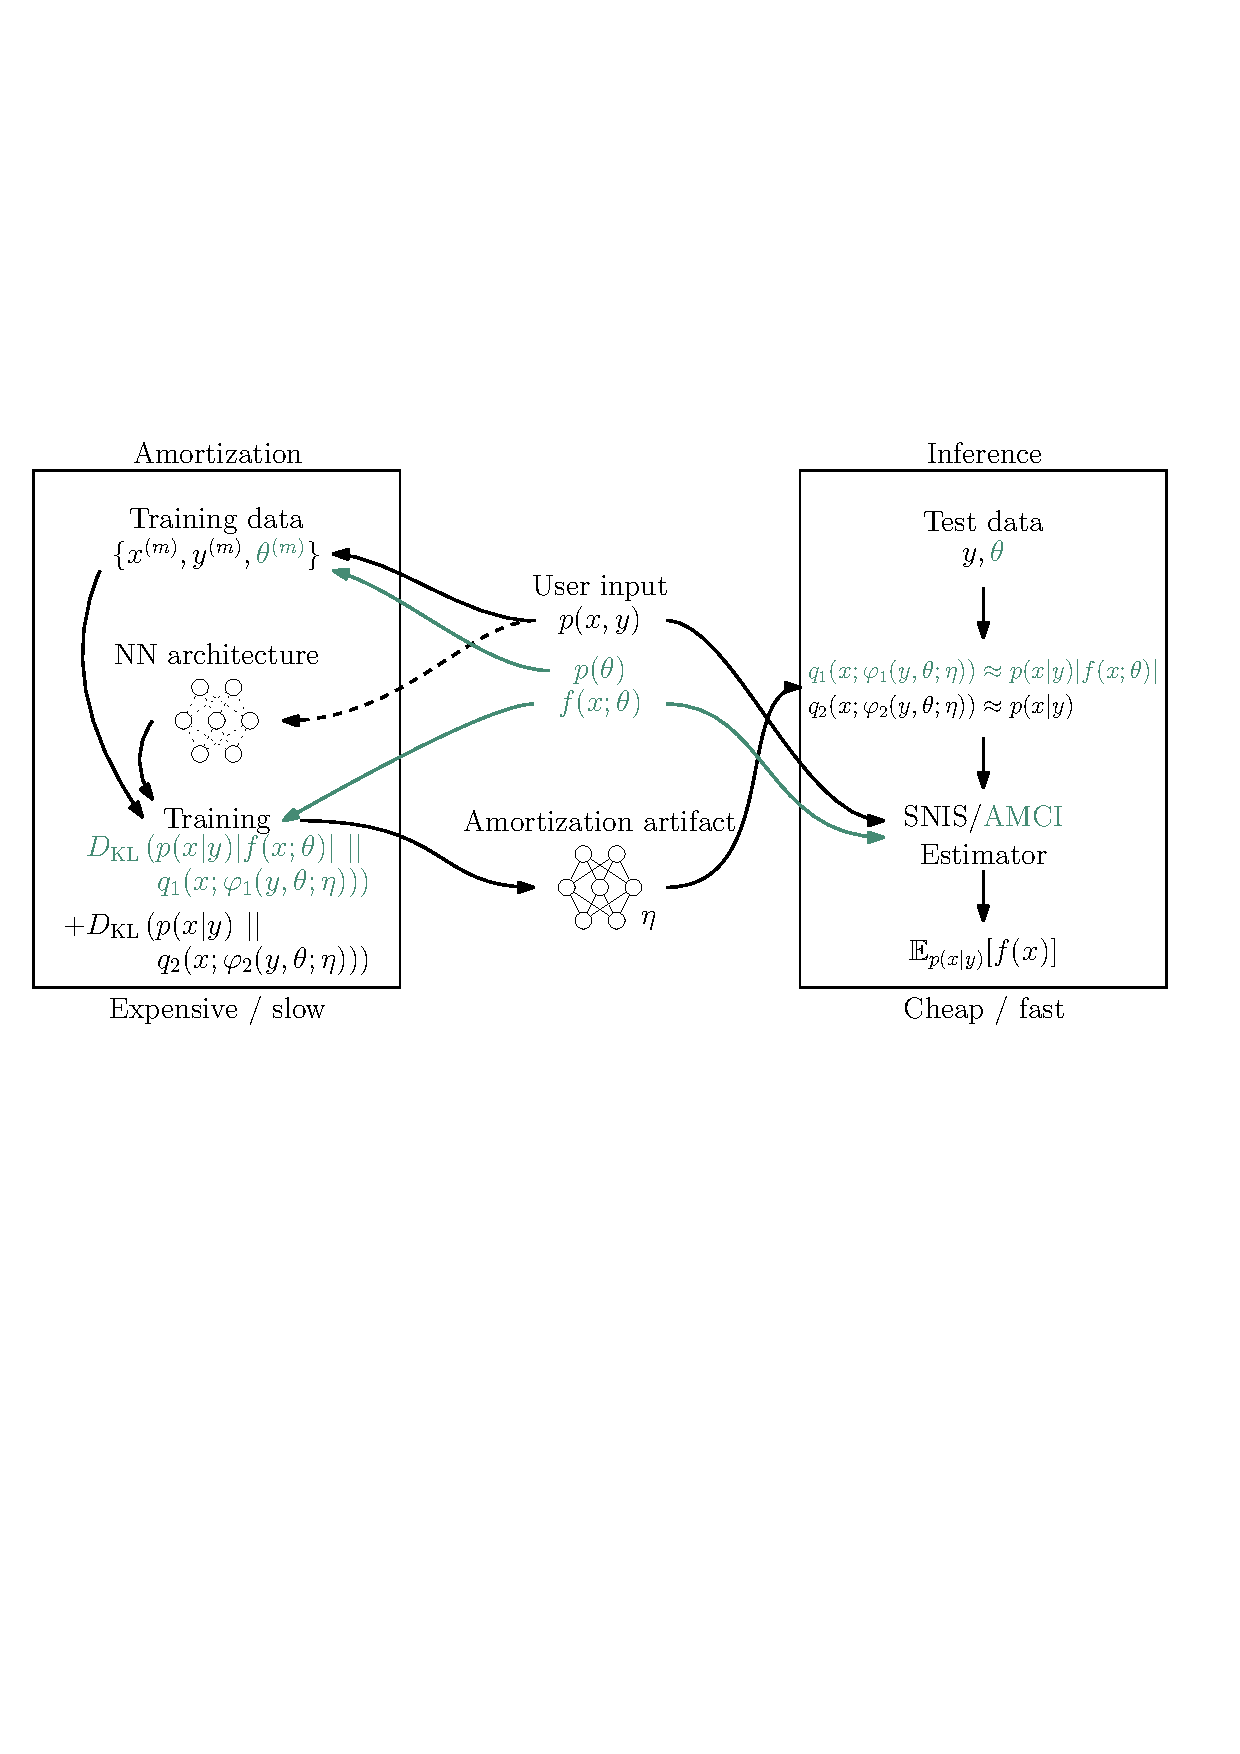
\includegraphics[width=0.8\linewidth]{figures/diagram.pdf}
%   \caption{
%   Schematic diagram of inference compilation for probabilistic programs. 
%   % Black elements refer to 
%   Original diagram courtesy of \citet{LeEtAl2016}.}
%   \label{fig:inf-amortization}
% \end{figure}
% \todo{describe the figure and tie it into the narrative}
% \todo{overall my research agenda is to continue contributing to the automation of inference amortization along those 3 questions and other extensions like AMCI}




% \subsection{Inference compilation vs ASVI}
% 
% In case of ASVI the model $p(x,y)$ is not fully specified by the user like in the inference compilation case
% when user provides the entire probabilistic program specifying the details of all of the stochastic and deterministic
% computation performed in the model.
% Instead, the user specifies the graphical model, i.e. factorization, of $p(x)$ and $p(y|x)$, 
% while the deterministic transformations of the sampled values are specified with a neural network with parameters $\theta$
% what is usually denoted as $p_\theta(y|x)$.
% 
% The process of designing of the inference network in both settings is similar, 
% but the more detailed our knowledge about the deterministic computation inside the generative model the larger is the opportunity we will be able to leverage it when designing an inference network.
% We touch upon this topic in \autoref{sec:design}.




\subsection{Designing the inference network}
\label{sec:design}

After we have decided on our model $p(x,y)$ in inference compilation or $p(x)$ and $p_\theta(y|x)$ in ASVI setting we need to design our inference network. 
That requires several design decisions that we elaborate on below:\\
1. The factorization of the approximate posterior $q(x|y)$: we need to decide about the graphical model $\mathcal{H}$ of the approximate posterior what implies it factorizes as $q(x|y)=\prod^N_i q_i(x_i\,|\,\text{Pa}_\mathcal{H}(x_i))$, this is equivalent to choosing the variational family in the classical variational inference setting;\\
2. The proposal distribution: typically we have to decide on a parametric distribution for each one of the factors $q_i$, but instead we could use more flexible density estimators that do not constrain us to parametric distribution families, e.g. normalizing flows \citep{RezendeMohamed2015}; \\
3. The function approximator: we need to decide how the parameters for the distribution or transformation in the normalizing flows are determined using a function approximator $\varphi$, usually this boils down to deciding about the architecture of a neural network $\varphi_i$ we are using to regress parameters for each of the factors 
$q_i(x_i\,|\,\text{Pa}_\mathcal{H}(x_i)) = q_i(x_i\,;\,\varphi_i(\text{Pa}_\mathcal{H}(x_i); \eta))$.\\


\subsubsection*{Factorization of the approximate posterior $q(x|y)$}

\todo{intro from Brooks' or Stuhlmueller's paper on why we need an inverse. 
do they explain what factorization or graphical models are at all?}
\todo{maybe some figure here}
\todo{add some information how inverses were derived in the past?}

The factorization of the approximate posterior $q(x|y)$ reflect the conditional independence assumptions between random variables we impose on the approximate posterior.
The more assumptions we impose the easier the problem is computationally, but the less expressive our approximate posterior $q(x|y)$ becomes and hence we make a coarser approximation.
The fewer assumption we impose the more expressive our approximate posterior $q(x|y)$ is, but it becomes more expensive to train and use.
Those assumptions are conveniently expressed using a framework called graphical modelling \citep{KollerFriedman2009}.

Such perspectives makes us consider a spectrum of assumptions we can impose on the approximate posterior.
On one end of this spectrum lies the one of coarsest approximations we can make called the mean field assumption -- assuming that the posterior factorizes into individual factors for each random variable $x_i$ without any dependencies between them, $q(x|y)=\prod^N_iq_i(x_i\,|\,y)$.
On the other end of this spectrum lies an autoregressive factorization which makes no assumptions since any joint distribution can always be factorized according to the probability chain rule $q(x|y)=\prod^N_iq_i(x_i\,|\,x_{<i},y)$.

What motivated the work in the first part of this report \citep{Webb2018} was the observation inspired by \citet{StuhlmullerEtAl2013} that if we impose more assumptions than those present in the generative model $p(x,y)$ we can make it impossible for our approximate posterior $q(x|y)$ to match the true posterior $p(x|y)$ no matter how flexible density estimator and how powerful function approximator we use.
In plain words the reason for this is that neural network that determines the parameters for the factor $q_i$ is not given all the necessary inputs (values of other random variables) to reconstruct the true posterior.
Even when our goal is not learning an accurate inference artifact but learning the model this effect is undesirable
% as limited capacity of the inference artifact forces the learnt model to adjust to this inaccurate inference hence limiting the capacity of the model itself, 
since because of the KL penalty term in the ELBO objective
$\mathcal{L}(y,q,p)=\log p(y)-KL(q(x|y) || p(x|y)) \le \log p(y)$ \citep{VAE}
optimizing under these assumptions tends to force the posterior $p_\theta(x|y)$ to satisfy the factorizing assumptions of the variational family $q$ \citep{FIVO}.

To alleviate that we introduced an algorithm that uses the graphical model $\mathcal{G}$ we assume for the generative model $p$ to search for a graphical model $\mathcal{H}$ for the approximate posterior which introduces as many assumptions as possible while not introducing any assumptions not present in the $p$, and hence not limit the expressivity of $q$ more than what is required to be able to match the true posterior.

We are not postulating that users should always use the factorization suggested by our method,
however we do recommend to use it as a guidance or a starting point before they decide to
introduce further assumptions into the inference network.

% Unlike mean-field and autoregressive factorizations, the factorizations produced by our method are very model-dependent and 
% we believe they provide more benefit to models with intricate graphical model structure.
% Compare VAE NaMI inverse which is just an autoregressive model with inverse of a binary tree.

% What is more -- you might wonder why we would like to limit the number of random variables on each factor of the factorization -- the goal of that is to limit the dimensionality of the conditioning set of RVs at each factor significantly.
% That translates into decreasing the dimensionality of the input to $\varphi_i$, we are analytically removing the inputs to the neural network that are unnecessary to determine the posterior.
% In case of structured models we would expect the dimensionality of the factors to be of the order $\mathcal{O}(1)$ as compared to $\mathcal{O}(N)$ for the autoregressive models where $N$ is the number of latent random variables in the model.
% We are not however circumventing one of the most significant issues of autoregressive models in general -- our lack of ability to parallelize the computation what at the moment is one of the bottlenecks in using methods such as Inverse Autoregressive Flows \citep{IAF} and Masked Autoregressive Flows \citep{MAF}, and is the motivation for the development of involved training strategies to combine the strengths of both techniques such as in \citep{ParallelWavenet}.
% However the total dimensionality of the latent variables in a model is often smaller than the that of the observed variables and in inference amortization we are only targeting the latent variables so there is still hope for sufficient efficiency for practical purposes.

% Major issue with using autoregressive NNs is that they need O(N) passes of a neural network.
% One of the issues that may arise when using NaMI inverses is a similar problem.
% Sampling from the inference network takes O(N) where N is the total dimensionality of the latent variables.
% In contrast the mean field assumption allows us to sample in O(1).
% This is also the issue with MAF.
% Maybe some kind of Parallel Wavenet approach would work here?
% NaMI inverses should take less time than autoregressive factorization but they will still be of order O(N).

\todo{can you add figures here? think when reading the draft and design the figure}

\todo{do people add auxiliary RVs that are later marginalized like $\hat{y}$ suggested here at the bottom \url{http://pyro.ai/examples/_static/img/ss_vae_zoo.png}?}



\subsubsection*{Proposal distribution}

In order to learn a proposal for each latent random variable in the model we need to choose what distribution to use on each factor $q_i$.
At the moment the most common approach in amortized inference is to use a parametric probability distribution with the parameters set by a neural network $\varphi_i(\text{Pa}_\mathcal{H}(x_i), \eta)$.
The simplest choice one could make for the distribution of a random variable is to use the same distribution family as in the generative model.
However, in many cases this distribution might not be flexible enough to match the true posterior well.
For example, for $x \in \mathbb{R}$ a mixture of gaussians is a more flexible choice than a single gaussian.

\todo{different requirements for proposal distribution for ASVI and inference compilation}

An alternative to using a parametric distribution might be a recently developed family of flexible density estimators called normalizing flows \citep{RezendeMohamed2015,IAF,MAF}.
Instead of requiring the distribution to have a closed form density expression normalizing flows take a sample $z$ from some tractable distribution, commonly standard normal, and transform it using a bijective (i.e. invertible) transformation $f: \mathbb{R} \mapsto \mathbb{R}$ (or series of such transformations) into a much more complex, possibly multi-modal, random variable $x=f(z)$.
We can still evaluate the probability density at any given point $x$ since we are able to compute the determinant of the Jacobian and apply the change of variables formula between the source of randomness $z$ and the final variable $x$ according to 
$p_x(x) = p_z(z) \left|
    \mathrm{det} \frac{
      \partial f^{-1}
    }{
      \partial z\
    }
  \right|$.
To make normalizing flows feasible, function $f$ is chosen so that the determinant of the Jacobian can be easily computed (e.g. by constraining $f$ such that the Jacobian is triangular), and it is additionally parameterized by $\eta$ which is tuned such that the output random variable $x$ match the desired distribution. In practice a part of $f(z, \eta)$ is constituted by a neural network with parameters $\eta$.
We also have to be able to take the derivative of the density with respect to the parameters $\eta$ what is required to train such a density estimator.
Normalizing flows are thus a promising tool for learning flexible proposals for the $\mathbb{R}^d$ domain.

% In this case we are only interested in proposals over one dimensional random variables since the factorization is decided on separately by the NaMI algorithm and hence we are not subject to the inefficiency of autoregressive flows in sampling (MAF) or density evaluation of an arbitrary point that was not obtained by sampling from it (IAF).

However, distributions in some other domains which are also relatively frequent in probabilistic modelling such as natural numbers $\mathbb{N}$, double bounded continuous $[a,b]$ or bounded continuous $\mathbb{R}^+$, are not addressed by the promise of normalizing flows and hence might require development of better density estimators for those domains.
Currently they are often addressed by the following parametric distributions, respectively: Poisson, Kumaraswamy or Beta, and Gamma.



\subsubsection*{Function approximator}
When using either the parametric distribution or normalizing flow as the proposal we need to choose the function approximator that is used to determine the parameters of the distribution or the transformation $f$ in normalizing flow.
Usually the function appoximator is a neural network and so our decision amounts to choosing its' architecture.

The probabilistic program specifies all of the deterministic transformations applied to the samples of the random variables in the generative model
what creates an opportunity to leverage that information in designing the architecture of the neural network by attempting to invert the computation in the generative model \citep{TavaresEtAl2016,TavaresEtAl2017}.
It is yet unclear if this approach will prove of practical use in the inference compilation setting.

Another possible route to automate the selection of the architecture would be to look into the neural architecture search literature \citep{ElskenEtAl2018,ZophLe2017,pham18a}.






% Methodology
% A good starting point for an attack on that problem is to limit the range of the models we will be able to run inference amortization on. One way to limit the range of models is to limit them to the finite-cardinality graphical models and attempt to invert their structure to guide the architecture of the neural network. That line of research was started by \citet{PaigeWood2016} and serves as our starting point that we plan to build upon.


% https://arxiv.org/pdf/1610.05735.pdf use the same ordering for their guide program as for the generative model as well as the same parametric family
% they also have some sort of optimization algorithm 
% 
% Tom
% >Unfortunately, there are two key stumbling blocks that often make it difficult for this idealized view of the Bayesian machine learning approach to be realized in practice. Firstly, a process known as Bayesian inference is required to solve the specified problems. This is typically a challenging task, closely related to integration, which is often computationally intensive to solve.
% 
% In terms of settings in which amortized inference is pursued there are 3 that should be named: 
% Bayesian Networks (BN) or Graphical Models (GM), i.e. models with deterministic number of random variables (RVs); 
% Deep Generative Models (DGMs) such as VAEs,
% Universal Probabilistic Programming.



\section{Research proposal}
There are several possible extensions and improvements to the existing inference amortization frameworks and systems. 
Below I list a few research directions that I am in good position to pursue.
The resulting projects vary in size, but each could yield a workshop or conference publication.
Some of them might end up being combined in a single paper for the purpose of publication.
I will provide more thorough description of each one below.
The list consists of the following themes and projects\\
\emph{Extensions to the inference compilation framework}\\
\textbf{A} \quad Amortized Monte Carlo Integration\\
\emph{Improvements and automation of inference compilation}\\
\textbf{B} \quad Normalizing flows as proposals for inference compilation\\
\textbf{C} \quad Choosing an inference network factorization in a data-driven way\\
% \textbf{E} \quad Making use of the information about the deterministic computations in the Bayesian networks and probabilistic programs\\
% \textbf{F} \quad Better ways of sampling from the model for the purpose of inference amortization\\
\emph{Applications of amortized inference in engineering, medicine and physical sciences}\\
\textbf{D} \quad Applications showcasing benefits of NaMI for models with rich structure\\




\subsubsection*{A \quad Amortized Monte Carlo Integration}
I am currently working on project A, Amortized Monte Carlo Integration.
We already have preliminary results published at UAI 2018 workshop on Uncertainty in Deep Learning \citep{golinski2018uai} and at International Conference on Probabilistic Programming 2018 \citep{golinski2018probprog} (without proceedings).
\todo{update page}
Please see page 22 for the copy of our UAI workshop paper.
Current plan is to perform additional experiments to showcase the utility of the method, establish a process to tune the hyperparameters and submit the work to AIStats 2018, and in case of rejection to ICML 2019.
 
% Since this project is in further stage of the development more details about it will follow in the next section.


% \subsubsection*{B \quad Probabilistic programming semantics for integration}
% Project A naturally leads to project B, establishing semantics for performing integration in probabilistic programming systems.
% % We present first thoughts and suggestions in \citep{golinski2018probprog}.
% % The semantics we propose are based on the semantics and program transformations introduced by \citet{rainforth2016bopp}.
% Specifically, we consider 
% how one might support it in Anglican~\citep{anglican}.
% Based on the query macro \defopt of~\citep{rainforth2016bopp}, 
% we introduce \clj{defint}.  Like \defopt, \clj{defint} adjusts Anglican's
% standard query macro, \defquery, by providing an series of symbols as an additional input.
% The role of this input is to identify the variables in the program which
% are function parameters $\theta$.  The value of the 
% function $f(x;\theta)$ is then given by the output of the query.
% We can thus express our previous
% example as follows
% \begin{lstlisting}[basicstyle=\ttfamily\small,frame=none]
% (defint example [y] [$\theta$]
%  (let [x (sample (normal 0 1))
%        $\theta$ (sample (uniform-continuous -5 5))]
%   (observe (normal x 1) y)
%   (> x $\theta$)))
% \end{lstlisting}
% The conditional distribution of this query corresponds to the distribution
% $p(x|y)p(\theta)$, while its output represents $f(x;\theta)$.  It thus
% contains all the information we require to carry out AMCI by estimating
% gradients of $\mathcal{J}$ and $\mathcal{J}'$:
% we can sample from $p(x,y)p(\theta)$ and have evaluations of
% $f(x;\theta)$ at these points.  Therefore by coupling the AMCI approach
% with the inference compilation approach introduced for Anglican
% in~\cite{LeEtAl2016}, we have everything required for
% training an ``integration compilation'' artifact.
% 
% The syntax used to identify which variables correspond to
% $\theta$ is necessary because
% a) we do not need to learn a proposal for $\theta$ and b) at test time, we need
% a way to fix the value of $\theta$.  The latter of this is simply dealt
% with using the maximum marginal likelihood transformation applied for \defopt
% in~\cite{rainforth2017thesis}.   This effectively removes the
% \sample statements for $\theta$, replacing them with identity functions
% and making $\theta$ an input to the program.  With this transformation and
% the appropriately adapted trained amortized proposals, we thus
% have a means of automatically applying AMCI at test time.


\subsubsection*{B \quad Normalizing flows as proposals for inference compilation}
Project C revolves around using normalizing flows as more flexible proposal distributions for inference compilation, as described in \autoref{sec:design}.
The most prevalent and challenging type of random variable to formulate a proposal for is a continuous variable with an unbounded support.
Current practice is to use a multimodal distribution such as Mixture of Gaussians with a fixed number of components $K$.
This choice may fail in several ways -- 
(1) there is no way for the proposal to match the true posterior if the posterior contains more than $K$ modes,
(2) the individual modes might not be very well approximated by a Gaussian, e.g. when they are highly asymmetric,
(3) the tails of the distribution might be heavier than those of Gaussian distribution.
Any of those scenarios might easily lead to a large (or even infinite) variance of our estimator, and hence to significant decrease in its sample efficiency.
An increasingly viable alternative to this approach is the growing family of flexible neural density estimation methods based on the idea of normalizing flow \citep{RezendeMohamed2015}.
I am planning to evaluate the utility of these methods, especially in the context of AMCI. 
% Currently the major difficulty of using normalizing flows for this purpose lies in the fact that methods allow either fast probability density evaluation at some data point $y$ (which is necessary for training) or the ability to efficiently sample (which is necessary at runtime).
% There are some attempts to circumvent this issue such as ParallelWavenet \citep{ParallelWavenet}, but anecdotal evidence suggests that approach is difficult to tune and train.
% Although I do not know of any successful attack on this problem yet I still deem it worthy to evaluate the utility of neural density estimators for amortized inference and its effect on sample efficiency of the final estimates even if we are not yet able to realize wall-time efficiency improvements in this way yet.

\subsubsection*{C \quad Choosing an inference network factorization in a data-driven way}
This project is a potential extension to the Natural Minimal Inverse (NaMI) method of inverting graphical models introduced by us in \citep{Webb2018}.
At the moment NaMI algorithm is forced to choose among multiple plausible faithful inverses of the generative graphical model and we use  heuristics to choose decide between those in principal equally faithful options.
% At the moment NaMI computes topological or reverse-topological sort orders, solves the draws between different orderings according to min-fill heuristic (i.e. minimizes the size of the cliques in the graph), computes two inverses and suggests to evaluate the performance of both.
My idea is to extend our current method to pick the factorization in a data-driven rather than heuristic way.
At a high level the new method would draw samples from the generative model and then use kernel density estimation to examine the form of the factors under different plausible factorizations. 
The `simpler` the forms of the factors are the easier they are to target with proposal distributions.
If a suitable measure of simplicity of a factor distribution is established it might be possible to further automate the process of choosing a suitable inference network factorization.


\subsubsection*{D \quad Applications showcasing the benefits of NaMI for models with rich structure}
At the moment we are lacking compelling examples showcasing the benefits of using our NaMI method.
We expect that our method yields most benefits for models with rich structure, and such can be found in the domains where
modelling is a prevalent tool of practice.
My plan is to seek suitable applications by looking for collaborators in engineering, finance, medicine or physical sciences.


\subsection{Preliminary schedule}
The following is a rough schedule for the rest of my DPhil degree, the milestones are pieces of work I intend to complete for relevant machine learning conferences.

\begin{table}[h!]
\begin{tabular}{lp{11cm}}
Present -- October 2019         & Further work on projects A\&B, submission to AIStats \\
October 2018 -- February 2019   & In case of rejection or delay further work on A\&B for submission to ICML, or investigation of project C \\
February 2019 -- May 2019       & Work on C or/and D depending on which one holds more promise, submission to NIPS or partial work to ICML workshop \\
May 2019 -- May 2020            & Reevaluation of available avenues for research and picking a new project \\
June 2020 -- October 2020       & Internship \\
October 2020 -- December 2020   & Writing up thesis
\end{tabular}
\end{table}


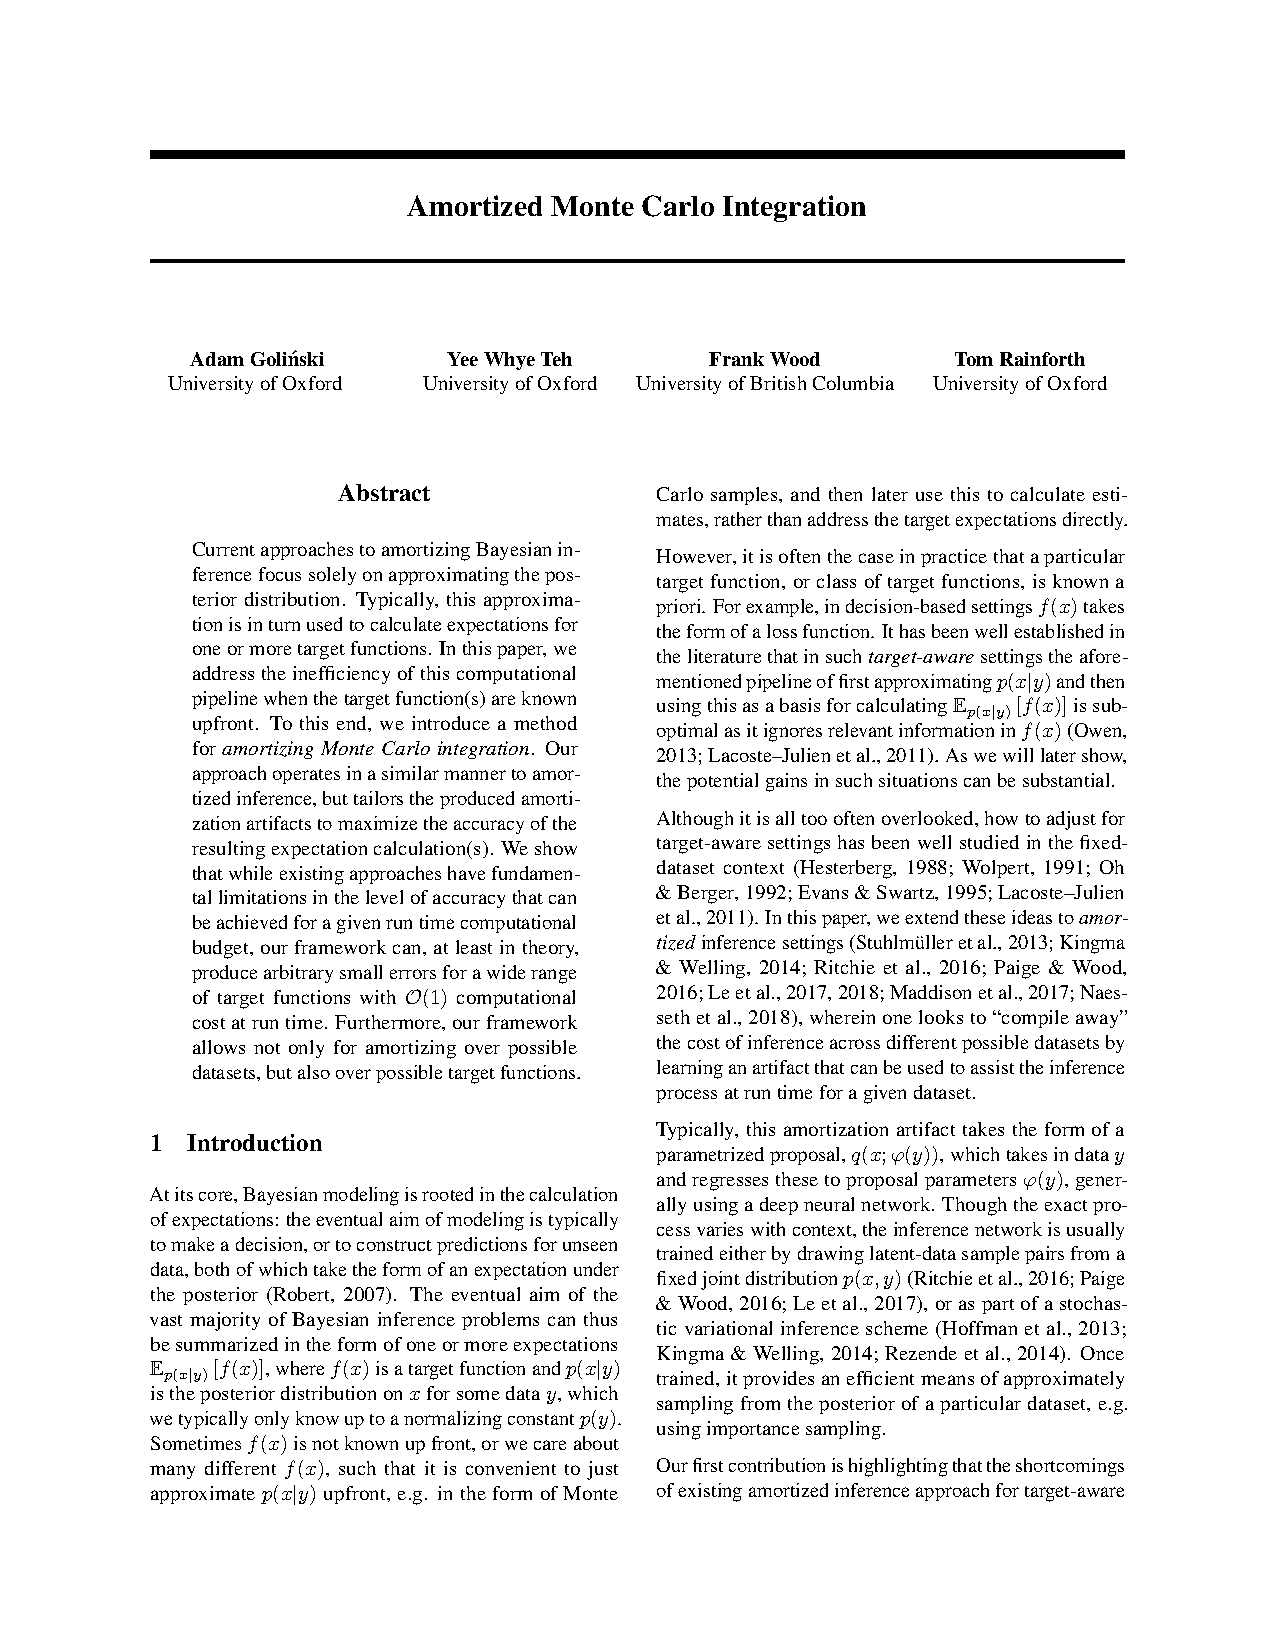
\includepdf[pages=-]{amci}

\newpage 
\bibliographystyle{plainnat}
\bibliography{bibliography/bibliography} 

% 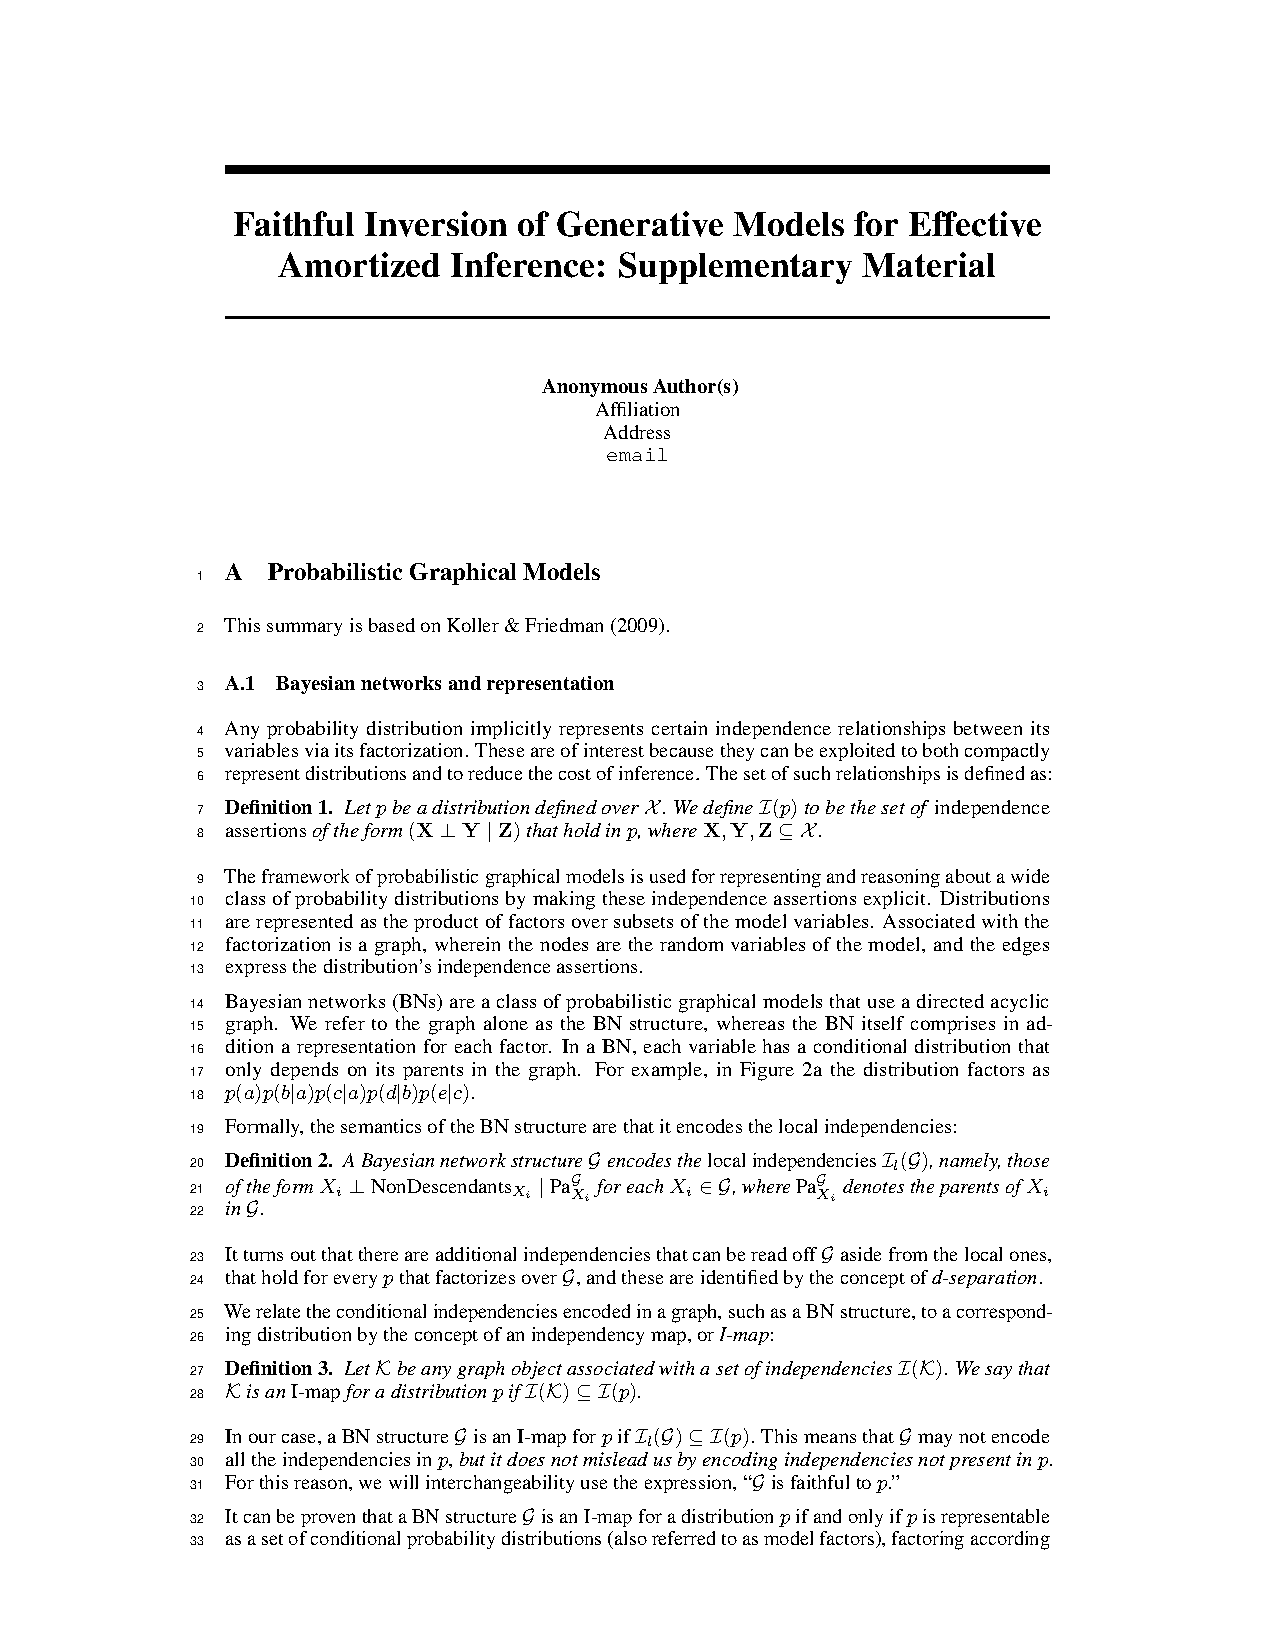
\includepdf[pages=-]{supplementary}

\end{document}
